% Illustrated system and receiver figure; compile: pdflatex fig_system.tex  ->  fig_system.pdf (included by main.tex)
\documentclass[tikz,border=2pt]{standalone}
\usepackage{amsmath,amssymb,bm}
\usetikzlibrary{arrows.meta,calc,positioning,shapes.geometric,decorations.pathmorphing,shadows}
\definecolor{cA}{HTML}{2a78d6}   % state 1 / ours
\definecolor{cB}{HTML}{eb6834}   % state 2
\definecolor{cG}{HTML}{1baf7a}
\definecolor{ink}{HTML}{0b0b0b}
\definecolor{mut}{HTML}{52514e}
\definecolor{pale}{HTML}{f3f2ee}
\begin{document}
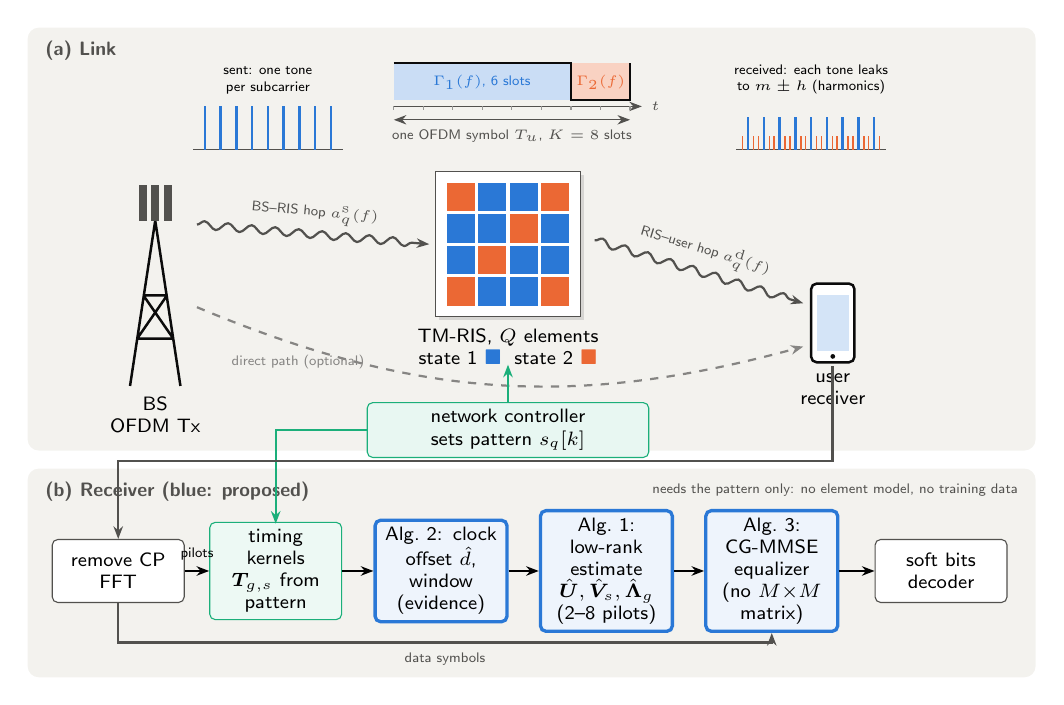
\begin{tikzpicture}[font=\sffamily\scriptsize, >={Stealth[length=1.6mm]},
  blk/.style={draw=mut, rounded corners=2pt, fill=white, align=center, inner sep=2.5pt, minimum height=8mm, text width=15mm},
  our/.style={blk, draw=cA, very thick, fill=cA!8},
  ray/.style={->, thick, mut, decorate, decoration={snake, amplitude=0.5mm, segment length=3mm, post length=1.6mm}}]

% ----------------------------------------------------------------- scene background
\fill[pale, rounded corners=4pt] (-0.4,-0.62) rectangle (12.4,4.75);
\node[anchor=north west, font=\sffamily\scriptsize\bfseries, mut] at (-0.3,4.7) {(a) Link};

% ----------------------------------------------------------------- base station (tower + antennas)
\begin{scope}[shift={(0.9,0.2)}]
  \draw[ink, line width=0.9pt] (0,0) -- (0.32,2.1) -- (0.64,0) (0.09,0.6) -- (0.55,0.6) (0.17,1.15) -- (0.47,1.15)
        (0.09,0.6) -- (0.47,1.15) (0.55,0.6) -- (0.17,1.15);
  \foreach \x in {0.16,0.32,0.48} \fill[mut] (\x-0.05,2.1) rectangle (\x+0.05,2.55);
  \node[below, align=center] at (0.32,-0.02) {BS\\OFDM Tx};
\end{scope}

% transmitted spectrum inset
\begin{scope}[shift={(1.7,3.2)}]
  \draw[mut] (0,0) -- (1.9,0);
  \foreach \i in {0,...,8} \draw[cA, line width=0.9pt] (0.15+0.2*\i,0) -- ++(0,0.55);
  \node[above, align=center, font=\sffamily\tiny] at (0.95,0.58) {sent: one tone\\per subcarrier};
\end{scope}

% ----------------------------------------------------------------- RIS panel (4x4, states at one instant)
\begin{scope}[shift={(4.9,1.2)}]
  \fill[white, drop shadow={opacity=0.25, shadow xshift=0.4mm, shadow yshift=-0.4mm}] (-0.12,-0.12) rectangle (1.72,1.72);
  \foreach \i in {0,...,3} \foreach \j in {0,...,3} {
    \pgfmathsetmacro{\st}{mod(\i+2*\j,3)==0 ? 1 : 0}
    \ifdim\st pt>0.5pt \fill[cB] (0.4*\i+0.02,0.4*\j+0.02) rectangle ++(0.36,0.36);
    \else \fill[cA] (0.4*\i+0.02,0.4*\j+0.02) rectangle ++(0.36,0.36); \fi }
  \draw[mut] (-0.12,-0.12) rectangle (1.72,1.72);
  \node[below, align=center] at (0.8,-0.15) {TM-RIS, $Q$ elements\\state 1 \textcolor{cA}{$\blacksquare$}\; state 2 \textcolor{cB}{$\blacksquare$}};
\end{scope}

% switching pattern inset (one OFDM symbol, K = 8 slots, D = 0.75)
\begin{scope}[shift={(4.25,3.75)}]
  \draw[->, mut] (0,0) -- (3.15,0) node[right, font=\sffamily\tiny] {$t$};
  \draw[ink, thick] (0,0.55) -- (2.25,0.55) -- (2.25,0.08) -- (3.0,0.08) -- (3.0,0.55);
  \fill[cA!25] (0,0.08) rectangle (2.25,0.55); \fill[cB!30] (2.25,0.08) rectangle (3.0,0.08+0.47);
  \draw[ink, thick] (0,0.55) -- (2.25,0.55) -- (2.25,0.08) -- (3.0,0.08) -- (3.0,0.55);
  \foreach \k in {0,...,8} \draw[mut!60] (0.375*\k,0) -- ++(0,-0.05);
  \node[font=\sffamily\tiny, text=cA] at (1.12,0.31) {$\Gamma_1(f)$, 6 slots};
  \node[font=\sffamily\tiny, text=cB] at (2.63,0.31) {$\Gamma_2(f)$};
  \draw[<->, mut] (0,-0.17) -- node[below, font=\sffamily\tiny] {one OFDM symbol $T_u$, $K=8$ slots} (3.0,-0.17);
\end{scope}

% ----------------------------------------------------------------- user equipment (phone)
\begin{scope}[shift={(9.55,0.5)}]
  \draw[ink, line width=0.9pt, rounded corners=2pt, fill=white] (0,0) rectangle (0.55,1.0);
  \fill[cA!20] (0.07,0.15) rectangle (0.48,0.85);
  \fill[ink] (0.275,0.075) circle (0.03);
  \node[below, align=center] at (0.275,-0.02) {user\\receiver};
\end{scope}

% received spectrum inset (each tone spread over harmonics)
\begin{scope}[shift={(8.6,3.2)}]
  \draw[mut] (0,0) -- (1.9,0);
  \foreach \i in {0,...,8} {
    \draw[cA, line width=0.9pt] (0.15+0.2*\i,0) -- ++(0,0.42);
    \draw[cB, line width=0.5pt] (0.15+0.2*\i+0.07,0) -- ++(0,0.17);
    \draw[cB, line width=0.5pt] (0.15+0.2*\i-0.07,0) -- ++(0,0.17); }
  \node[above, align=center, font=\sffamily\tiny] at (0.95,0.58) {received: each tone leaks\\to $m\pm h$ (harmonics)};
\end{scope}

% ----------------------------------------------------------------- propagation hops
\draw[ray] (1.75,2.25) -- node[above, sloped, font=\sffamily\tiny] {BS--RIS hop $a^{\rm s}_q(f)$} (4.7,2.0);
\draw[ray] (6.8,2.05) -- node[above, sloped, font=\sffamily\tiny] {RIS--user hop $a^{\rm d}_q(f)$} (9.45,1.25);
\draw[->, thick, mut!70, dashed] (1.75,1.2) to[bend right=19] node[below, font=\sffamily\tiny, pos=0.16] {direct path (optional)} (9.45,0.7);

% control link (pattern)
\node[blk, text width=34mm, minimum height=5mm, fill=cG!10, draw=cG] (ctl) at (5.7,-0.36) {network controller sets pattern $s_q[k]$};

% ----------------------------------------------------------------- receiver chain
\fill[pale, rounded corners=4pt] (-0.4,-3.5) rectangle (12.4,-0.85);
\node[anchor=north west, font=\sffamily\scriptsize\bfseries, mut] at (-0.3,-0.9) {(b) Receiver (blue: proposed)};
\node[blk]  (fft) at (0.75,-2.15) {remove CP\\FFT};
\node[blk, draw=cG, fill=cG!8] (ker) at (2.75,-2.15) {timing kernels\\$\bm T_{g,s}$ from\\pattern};
\node[our]  (off) at (4.85,-2.15) {Alg.~2: clock\\offset $\hat d$, window\\(evidence)};
\node[our]  (est) at (6.95,-2.15) {Alg.~1: low-rank\\estimate $\hat{\bm U},\hat{\bm V}_s,\hat{\bm\Lambda}_g$\\(2--8 pilots)};
\node[our]  (eq)  at (9.05,-2.15) {Alg.~3: CG-MMSE\\equalizer\\(no $M{\times}M$ matrix)};
\node[blk]  (dec) at (11.2,-2.15) {soft bits\\decoder};
\draw[->, thick] (fft) -- node[above, font=\sffamily\tiny] {pilots} (ker);
\draw[->, thick] (ker) -- (off); \draw[->, thick] (off) -- (est); \draw[->, thick] (est) -- (eq); \draw[->, thick] (eq) -- (dec);
\draw[->, thick, mut] (fft.south) -- ++(0,-0.5) -| node[below, pos=0.25, font=\sffamily\tiny] {data symbols} (eq.south);
\draw[->, thick, cG] (ctl.west) -| (2.75,-1.55);
\draw[->, thick, cG] (ctl.north) -- (5.7,0.47);
\draw[->, thick, mut] (9.82,0.45) |- (0.75,-0.75) -- (fft.north);
\node[font=\sffamily\tiny, text=mut, anchor=north east] at (12.3,-0.92) {needs the pattern only: no element model, no training data};
\end{tikzpicture}
\end{document}
